\section{Cryptage du mot de passe}

Lors du déroulement du jeu nous allons avoir besoin de stocker le mot de passe du joueur. Pour cela, nous avons pensé qu'il était préférable d'encrypter ce mot de passe lors de son stockage. \\
Nous avons ainsi chercher différentes méthodes pour effectuer l'encryptage du mot de passe. 

\subsection{Fonctions SQL}

Dans le langage SQL, la fonction MDA5() permet de chiffrer une chaîne de caractère en un entier hexadécimal de 32 caractères. \\
L'algorithme MDA() est une fonction de hachage cryptographique qui calcule à partir d'une chaîne de caractère son empreinte avec une probabilité très forte que deux empreintes soient différentes. Depuis 2004, une équipe chinoise a découvert des collisions complètes et MD5 n'est donc plus considéré comme sur au sens cryptographique. \\

La fonction SQL SHA1() permet de chiffrer une chaîne de caractère sous la forme d'un chaîne de caractères de 40 caractères. SHA1 est également une fonction de hachage cryptographique. Elle a l'avantage d'être considéré comme sur contrairement à MDA(). 



\subsection{Jasypt}
Jasypt est une librairie java qui permet d'encrypter facilement les mots de passe avec une une grande sécurité. \\
Jasypt possede les avantages suivants :
\begin{itemize}
\item il permet de choisir la fonction de hachage que nous souhaitons (MDA ou SHA par exemple)
\item il ajoute un salage au mot de passe qui permet d'avoir deux mots de passe cryptés différents pour le même mot de passe de départ
\item il applique un nombre aléatoire de fois notre fonction de hachage (nombre > 1000 pour rendre plus difficile les attaques)
\end{itemize}  

Nous pouvons résumer l'algorithme de chiffrement de Jasypt comme suit :\\
\begin{figure}[!h]
  \center
  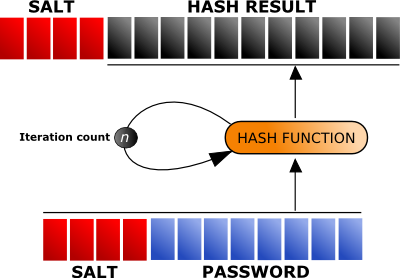
\includegraphics[scale=0.7]{../graph/passwordEncryption.png} \\
  \caption{Schéma simple du fonctionnement de Jasypt - http://www.jasypt.org/howtoencryptuserpasswords.html}
\end{figure}
Le code pour encrypter le mot de passe est très simple, il nous suffit de créer un objet de type ConfigurablePasswordEncryptor, de définir l'algorithme de chiffrement. La méthode setPlainDigest nous permet avec l'argument false de choisir la méthode la plus sure avec un salage et un nombre d'itération aléatoire pour notre fonction de hachage. Enfin il ne nous reste plus qu'a appeler la méthode encryptPassword qui nous renvoie notre mot de passe encrypté à partir d'un mot de passe donné en entrée. 
\begin{lstlisting}
 ConfigurablePasswordEncryptor passwordEncryptor = new ConfigurablePasswordEncryptor();
 passwordEncryptor.setAlgorithm( ALGO_CHIFFREMENT );
 passwordEncryptor.setPlainDigest( false );
 String motDePasseChiffre = passwordEncryptor.encryptPassword( motDePasse );
\end{lstlisting} 


De même que pour vérifier que notre mot de passe correspond au mot de passe chiffré il existe une méthode qui nous renvoie vraie en cas de correspondance :

\begin{lstlisting}
passwordEncryptor.checkPassword(motDePasse, motDePasseChiffre )
\end{lstlisting}


\subsection{Notre choix}
L'inconvénient d'utiliser les fonctions de SQL est que l'on choisi une manière de crypter dépendante de notre base de données. Si nous décidons de changer notre manière de stocker notre base de données nous devrons ainsi trouver une nouvelle fonction. \\

Nous avons donc choisi d'utiliser Jasypt pour encrypter notre mot de passe. Cette librairie a l'avantage de nous permettre d'encrypter uen chaîne de caractère de manière relativement sure sans avoir de grandes compétences en cryptographie. En effet, nous ne connaissons pas en détail le fonctionnement de l'algorithme de cryptage mais avons simplement une idée globale de son fonctionnement. \\

Nous avons choisi comme fonction de hachage (ALGOCHIFFREMENT) SHA car nous avons que MDA n'est plus sur. Une fois l'encryptage du mot de passe effectué nous obtenons une chaîne de caractères de taille 56.